\begin{figure}[b!]
    \vspace{-3mm}
    \centering
    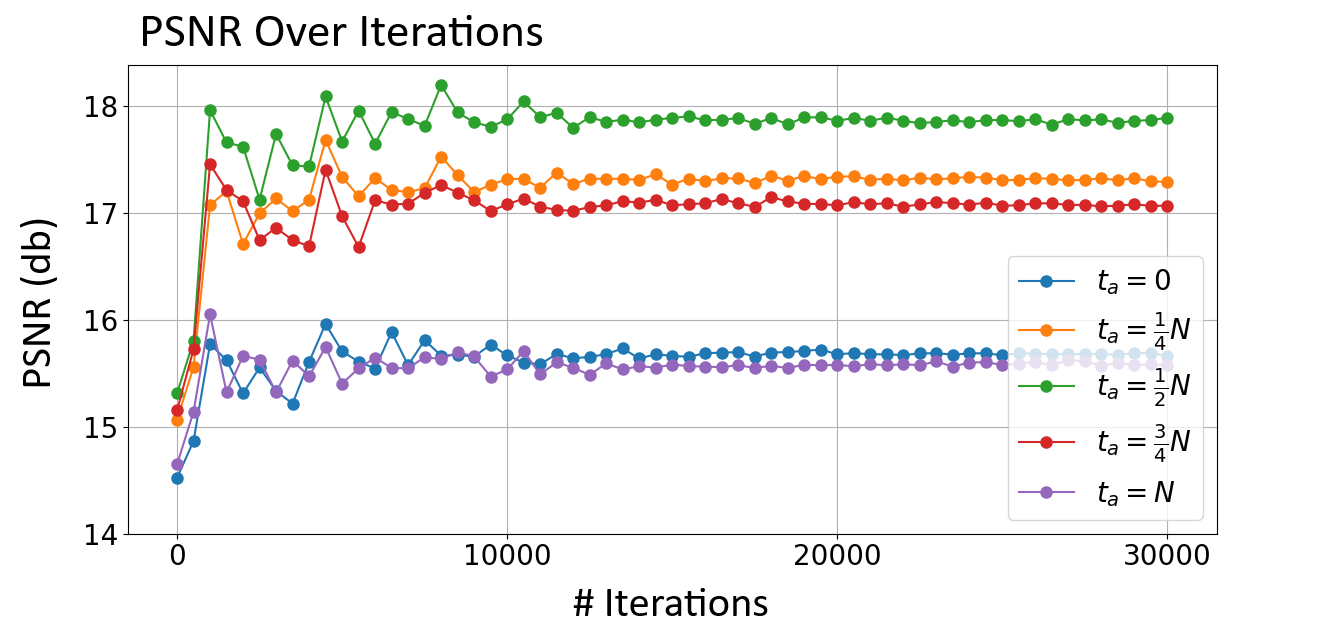
\includegraphics[width=0.49\textwidth, trim=0 2 0 16.5mm,  % left bottom right top
        clip]{X4K_data/figure (1).png} % Path to your first image
    
    \caption{Comparison of PSNR in the five models described in Sec. V-B. Performing a grid search on the possible anchor point location yielded different networks with varying accuracies. These experiments support the use of the anchor point $\frac{N}{2}$ for the real-world scenes.}

    % Comparison of PSNR in the five models described in Sect. 5.B. Each model, with a different anchor point, is represented by a different color on the graph. We validated our theory for anchor points for general scenes. Performing a grid search on the possible anchor point location yielded different networks with varying accuracies. This experiments supported the use of the anchor point $\frac{N}{2}$ for the real-world scenes.
    \vspace{-2mm}
    \label{fig:PSNR_X4K}
\end{figure}